% Anatomy of the pulmonary airways -- structure, function, nomenclature, what imaging resolves,
% and how the complete tree is estimated. Subsection of "Background" (sections/02-background.tex).
% Figures in figures/airway_*.png are cropped from the cited publications (captions removed);
% figures/airway_bronchial_alveolar_trees.jpg is the Anatomy.app image, used unmodified.

\subsection{Anatomy of the pulmonary airways}  % what the object of this work is
\label{sec:anatomy}                      % \secref{sec:anatomy}

The pulmonary airways form a branching tree of tubes that carries air from the trachea to the
alveoli, where gas exchange takes place (Figure~\ref{fig:anatomy_overview}). This subsection summarizes how the tree is organized,
how its branches are named, which part of it current imaging can resolve, and how the part
that cannot be imaged is estimated.

\begin{figure}[htbp]                     % overview of the bronchial and alveolar trees
  \centering                             % center the figure
  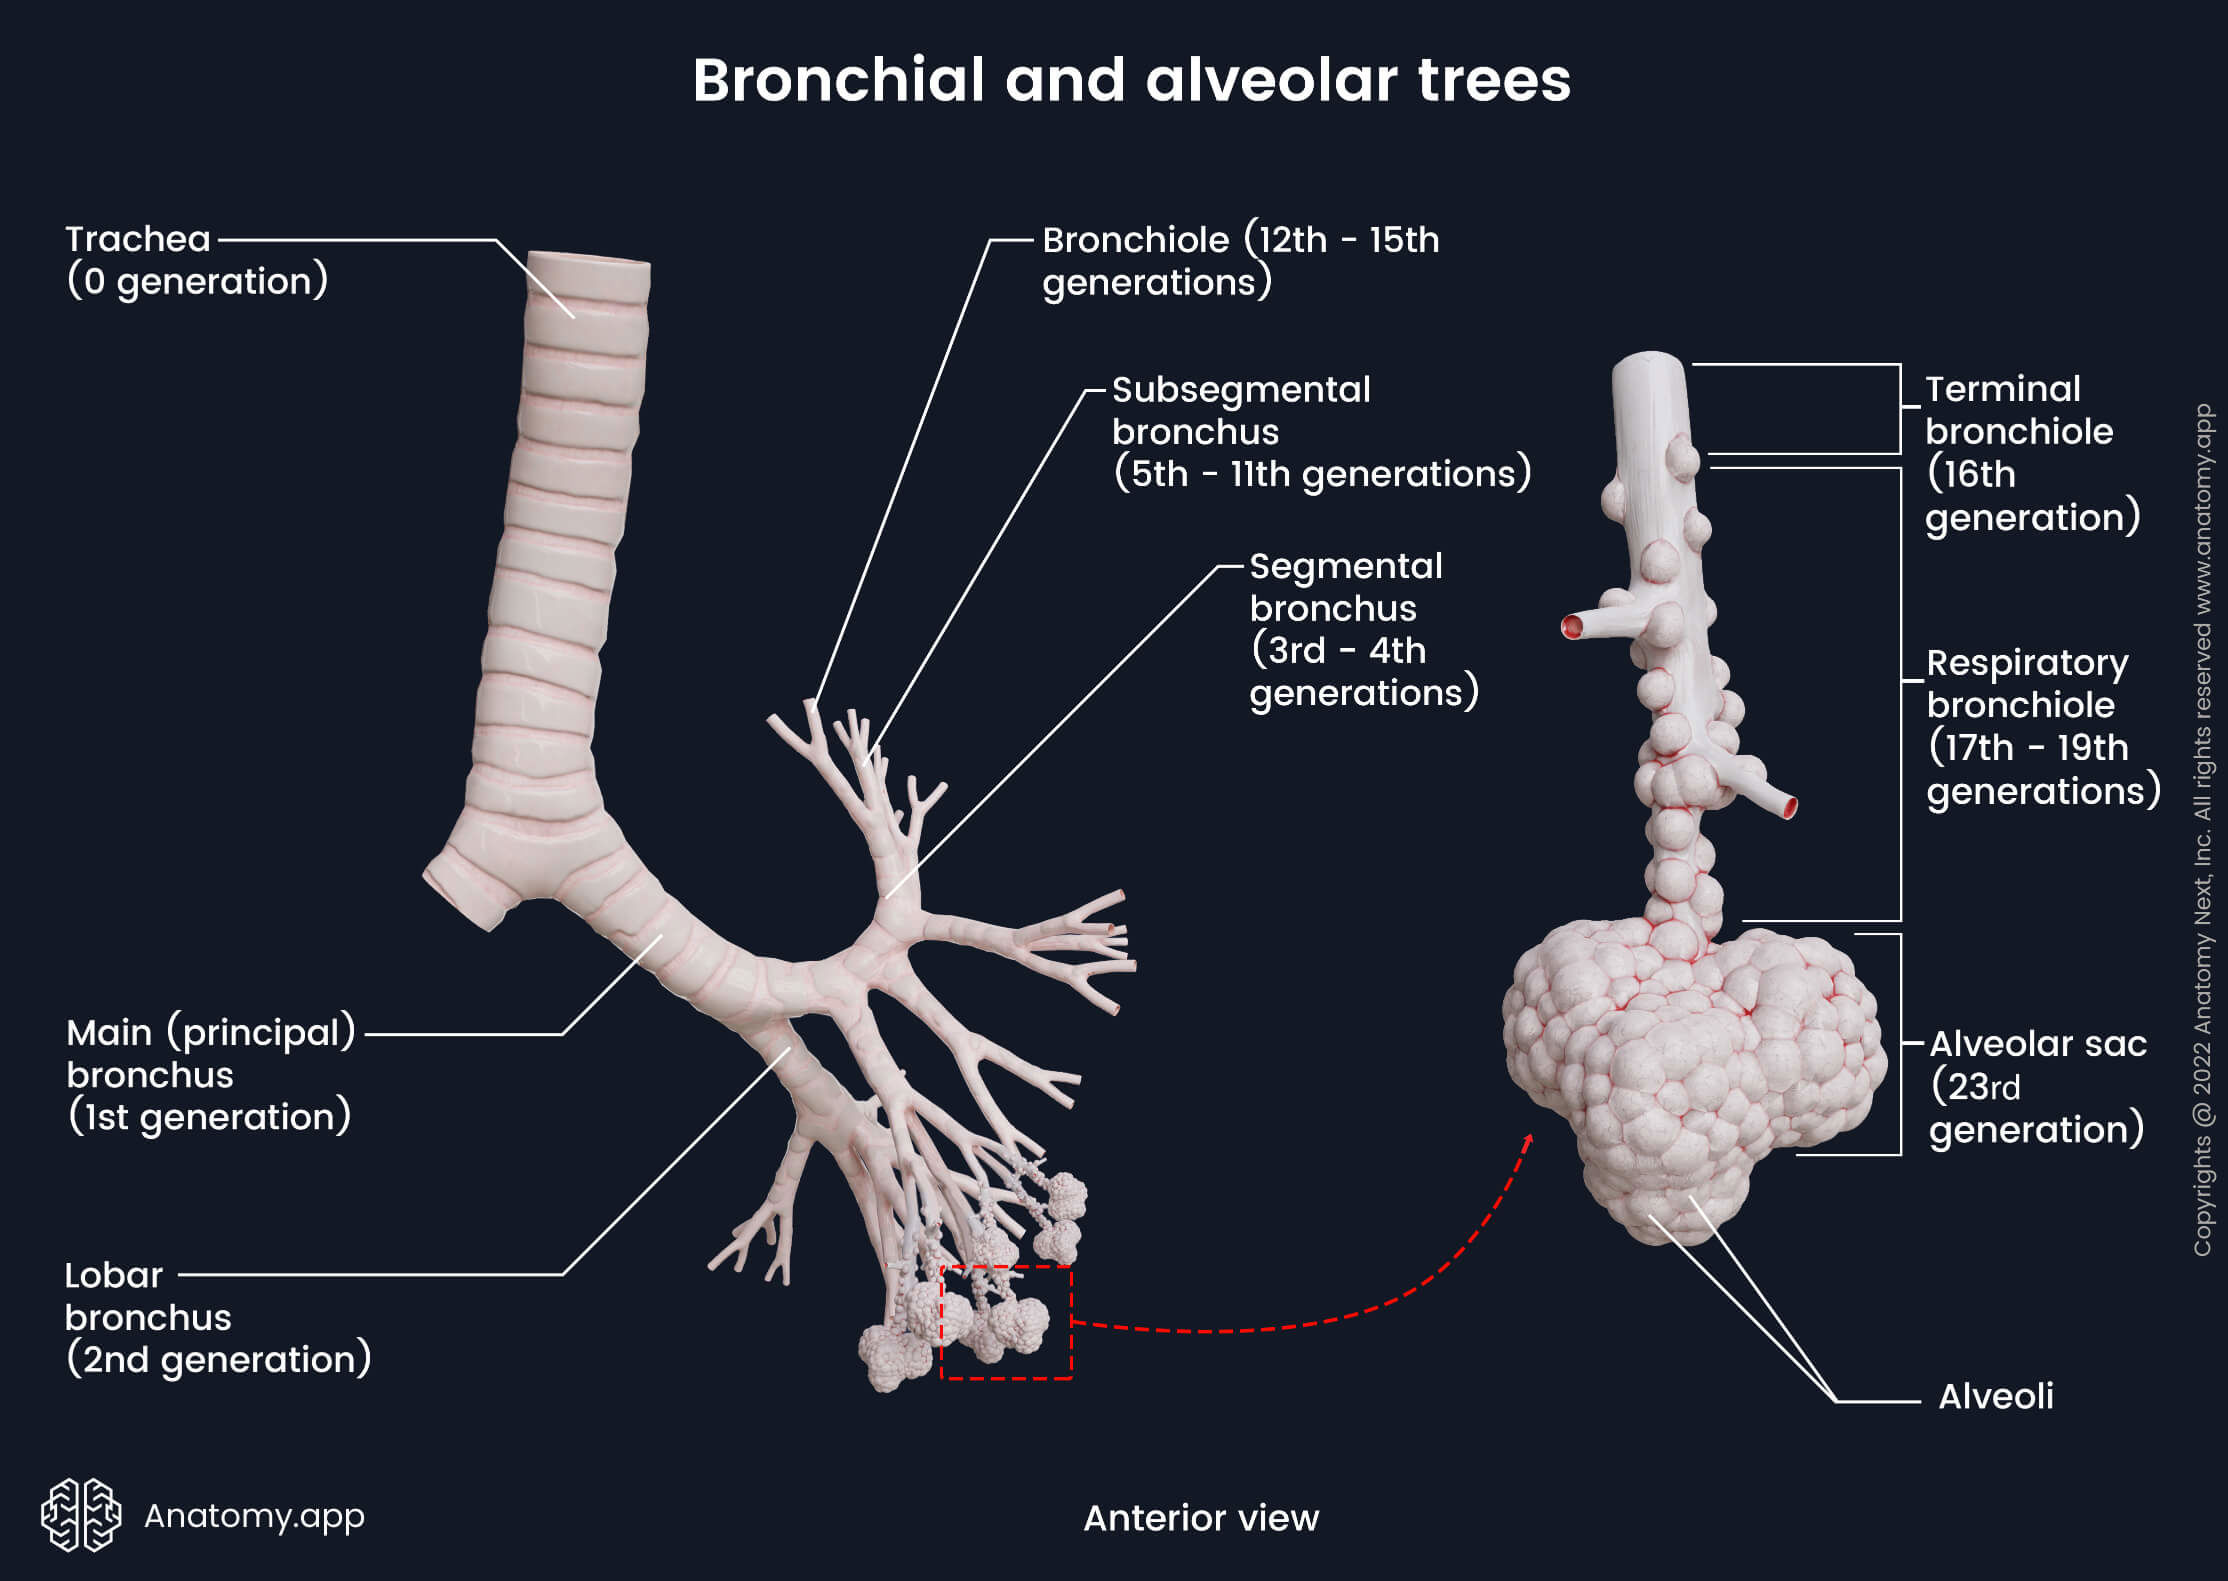
\includegraphics[width=\textwidth]{figures/airway_bronchial_alveolar_trees.jpg}  % user-supplied image, unmodified
  \caption{Bronchial and alveolar trees (anterior view). The conducting airways run from the
           trachea (generation 0) through the main, lobar, segmental and subsegmental bronchi and
           the bronchioles to the terminal bronchioles (generation 16); the enlarged detail shows
           the respiratory zone, with respiratory bronchioles (generations 17--19) and an
           alveolar sac (generation 23) covered with alveoli. The generation ranges differ
           slightly between sources (compare Table~\ref{tab:weibel_generations}). Image
           \copyright~2022 Anatomy Next, Inc., reproduced from Anatomy.app \cite{anatomyapp}.}
  \label{fig:anatomy_overview}           % referenced as Figure~\ref{fig:anatomy_overview}
\end{figure}

\paragraph{Structure and function.}      % conducting vs respiratory zone, generations
Starting from the trachea, each airway divides into daughter branches of smaller diameter and
length. The branching level is counted in \emph{generations}: in the classical symmetric model
of \citet{weibel1963}, the trachea is generation~0 and every airway splits into two, so that
generation $z$ contains $2^z$ airways and the tree ends after 23 generations
(Table~\ref{tab:weibel_generations}). Generations 0 to 16 form the \emph{conducting zone}:
the trachea, bronchi and bronchioles down to the terminal bronchioles. They take no part in gas
exchange; they conduct, warm, humidify and filter the inspired air, and their volume forms the
anatomical dead space. Generations 17 to 23 form the \emph{respiratory zone}, whose
respiratory bronchioles, alveolar ducts and alveolar sacs carry the alveoli in which oxygen and
carbon dioxide diffuse between air and blood \cite{weibel1963}. Because the number of airways
doubles at each generation while their diameter shrinks by only about a fifth, the total
cross-section grows quickly towards the periphery and the air slows down, so that transport in
the deepest generations is dominated by diffusion. The bronchi are supported by cartilage,
whereas the bronchioles are not; the non-cartilaginous airways with an internal diameter below
about 2~mm, found from roughly the eighth generation onwards, are called the \emph{small
airways} \cite{burgel2013small}. Real airway trees are not symmetric: the two daughters of a
bifurcation usually differ in diameter, length and angle, and the number of generations
between the trachea and a terminal bronchiole varies from one path to another
\cite{horsfield1971models,kitaoka1999}.

\begin{table}[htbp]                      % Weibel's symmetric model, grouped by zone
  \centering                             % center the table
  \small                                 % slightly smaller font so the table fits
  \caption{Airway generations in the symmetric model of \citet{weibel1963}. Diameters are
           approximate model values for an adult lung; real trees are asymmetric, so the
           correspondence between generation and airway type is only indicative. The last
           column indicates which airways clinical CT can resolve
           \cite{burgel2013small}.}
  \label{tab:weibel_generations}         % referenced as Table~\ref{tab:weibel_generations}
  \begin{tabular}{llccc}                 % zone, airway, generation, diameter, CT
    \toprule
    Zone & Airway & Generation $z$ & Diameter (mm) & Clinical CT \\
    \midrule
    Conducting  & Trachea                & 0       & 18        & Yes \\
                & Main bronchi           & 1       & 12        & Yes \\
                & Lobar bronchi          & 2       & 8         & Yes \\
                & Segmental bronchi      & 3       & 6         & Yes \\
                & Subsegmental bronchi   & 4       & 4.5       & Yes \\
                & Small bronchi          & 5--11   & 3.5--1.1  & Partly \\
                & Bronchioles            & 12--15  & 1.0--0.7  & No \\
                & Terminal bronchioles   & 16      & 0.6       & No \\
    \midrule
    Respiratory & Respiratory bronchioles & 17--19 & 0.5       & No \\
                & Alveolar ducts         & 20--22  & 0.4       & No \\
                & Alveolar sacs          & 23      & 0.4       & No \\
    \bottomrule
  \end{tabular}
\end{table}

\paragraph{Anatomical nomenclature.}     % lobes and segments (Table)
Below the generation count, airways are named after the lung region they supply. At the carina
the trachea divides into the right and left main bronchi. The right lung has three lobes
(upper, middle and lower) and the left lung two (upper, including the lingula, and lower), each
supplied by a lobar bronchus. The lobar bronchi divide into \emph{segmental bronchi}, each
ventilating one bronchopulmonary segment. The right lung has ten segmental bronchi, RB1 to
RB10; in the left lung, the apical and posterior segments and the anterior and medial basal
segments usually share a bronchus (LB1+2 and LB7+8), which gives eight segmental bronchi
(Table~\ref{tab:segmental_bronchi}). This nomenclature goes back to systematic studies of the
bronchopulmonary segments \cite{boyden1949}, which also documented how frequent anatomical
variations are, for example trifurcations of the right upper lobe bronchus in almost half of
the subjects \cite{boyden1949} and of the left upper division and lower lobar bronchi in about
a fifth \cite{zhao2009}. The $10+8=18$ segmental bronchi, together with the trachea and main
bronchi, are the classes predicted by the labelling model used in this work
(\secref{sec:labeling}) \cite{xie2025}.

\begin{table}[htbp]                      % segmental bronchi per lobe
  \centering                             % center the table
  \small                                 % slightly smaller font so the table fits
  \caption{Lobar and segmental bronchi of the human airway tree.}
  \label{tab:segmental_bronchi}          % referenced as Table~\ref{tab:segmental_bronchi}
  \begin{tabular}{lll}                   % lung, lobe, segmental bronchi
    \toprule
    Lung  & Lobe   & Segmental bronchi \\
    \midrule
    Right & Upper  & RB1 apical, RB2 posterior, RB3 anterior \\
          & Middle & RB4 lateral, RB5 medial \\
          & Lower  & RB6 superior, RB7 medial basal, RB8 anterior basal, \\
          &        & RB9 lateral basal, RB10 posterior basal \\
    \midrule
    Left  & Upper  & LB1+2 apicoposterior, LB3 anterior, \\
          &        & LB4 superior lingular, LB5 inferior lingular \\
          & Lower  & LB6 superior, LB7+8 anteromedial basal, \\
          &        & LB9 lateral basal, LB10 posterior basal \\
    \bottomrule
  \end{tabular}
\end{table}

\paragraph{What current imaging can resolve.}  % CT resolution limits
Clinical CT has a spatial resolution of about 0.6 to 1~mm, which allows direct assessment of
airways down to a diameter of about 2 to 2.5~mm; normal bronchioles are not visible
\cite{burgel2013small}. The datasets used in this work fall in this range, with in-plane
resolutions of 0.5 to 0.92~mm and slice thicknesses of 0.45 to 1~mm for ATM'22
(\secref{sec:atm22}). In Weibel's model, the airway diameter falls below 2~mm around the eighth
generation (Table~\ref{tab:weibel_generations}); in real, asymmetric trees this happens
earlier along many paths, and in patients with COPD most sixth-generation airways of the
apical and posterior basal segments are already narrower than 2~mm \cite{tanabe2019peripheral}.
A lumen that spans only one or two voxels is also blurred by the partial volume effect, so
segmentations lose branches and suffer breakages towards the periphery \cite{zhang2024}.
Ultra-high-resolution CT, with 0.25~mm slices and $1024 \times 1024$ matrices, can measure
airways of 1 to 2~mm in vivo \cite{tanabe2018uhrct,tanabe2019peripheral}, and smaller airways
have so far been studied mainly with histology and micro-CT on excised lungs
\cite{tanabe2018uhrct}. MRI, with hyperpolarized gases or ultrashort echo times, avoids
ionizing radiation but has a lower resolution and reaches at most the segmental and
subsegmental bronchi \cite{lewis2005,genkin2024}. In practice, an airway tree segmented from CT
therefore contains the central airways and a limited number of further generations, only a
small fraction of the tens of thousands of terminal bronchioles of the real tree.

\paragraph{Estimating the complete tree.}  % models beyond CT resolution
Because the peripheral airways cannot be imaged in vivo, the complete tree is estimated with
models. Anatomically based models grow the tree inside the lung volume with fractal-like or
volume-filling rules that reproduce morphometric data \cite{kitaoka1999,tawhai2000}
(Figure~\ref{fig:anatomy_fractal}). Patient-specific models combine both: the lobes and the
central airways are segmented from CT, and the tree beyond CT resolution is generated inside
each lobe, guided by the resolved airways and the lobar boundaries
\cite{tawhai2004,bordas2015,pennati2024modeling} (Figure~\ref{fig:anatomy_pipeline}). AVATREE
follows the same idea and can extend a CT-derived tree to any number of generations
\cite{nousias2020avatree} (Figure~\ref{fig:anatomy_generations}). The comparison between the
central airways and the estimated tree in these figures shows how small the CT-visible part of
the airway tree is. All the airway trees used in this work, and therefore all the
representations and models of the following sections, are limited to this CT-resolved part.

\begin{figure}[htbp]                     % fractal-like 3D model of the complete tree
  \centering                             % center the figure
  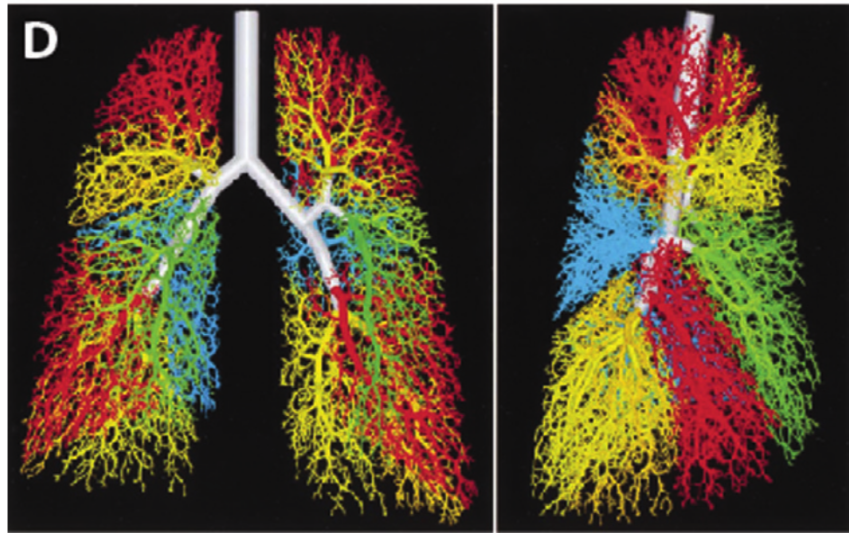
\includegraphics[width=0.75\textwidth]{figures/airway_fractal_model.png}  % front and side views
  \caption{Three-dimensional model of the human airway tree generated with fractal-like rules,
           in front and side views. The model contains more than 50,000 branches and matches
           morphometric data from human lungs. Reproduced from
           \citet{varner2017computational}, who adapted it from earlier work.}
  \label{fig:anatomy_fractal}            % referenced as Figure~\ref{fig:anatomy_fractal}
\end{figure}

\begin{figure}[htbp]                     % CT -> segmentation -> complete tree
  \centering                             % center the figure
  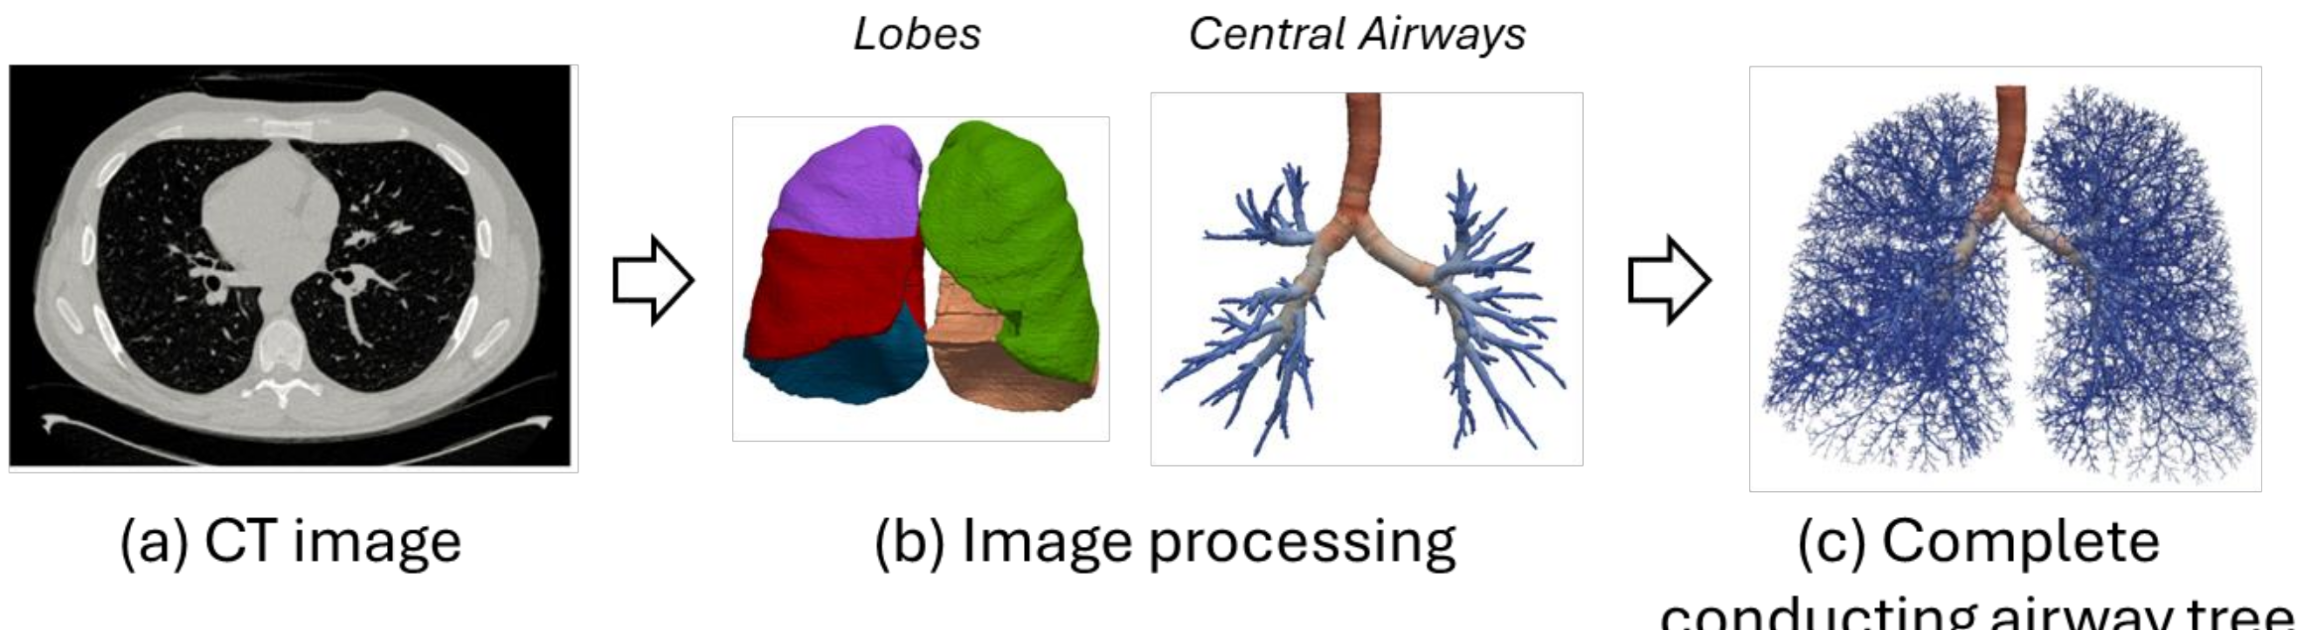
\includegraphics[width=\textwidth]{figures/airway_ct_to_complete_tree.png}  % three-step pipeline
  \caption{Patient-based model of the complete conducting airway tree: (a) CT image; (b) lobes
           and central airways segmented from the CT image; (c) airway tree beyond CT
           resolution generated with a lobe-filling algorithm, colour-coded by airway radius.
           Reproduced from \citet{pennati2024modeling}, who adapted it from earlier work.}
  \label{fig:anatomy_pipeline}           % referenced as Figure~\ref{fig:anatomy_pipeline}
\end{figure}

\begin{figure}[htbp]                     % 12 vs 23 estimated generations
  \centering                             % center the figure
  \begin{minipage}[b]{0.49\textwidth}    % left panel
    \centering                           % center inside the panel
    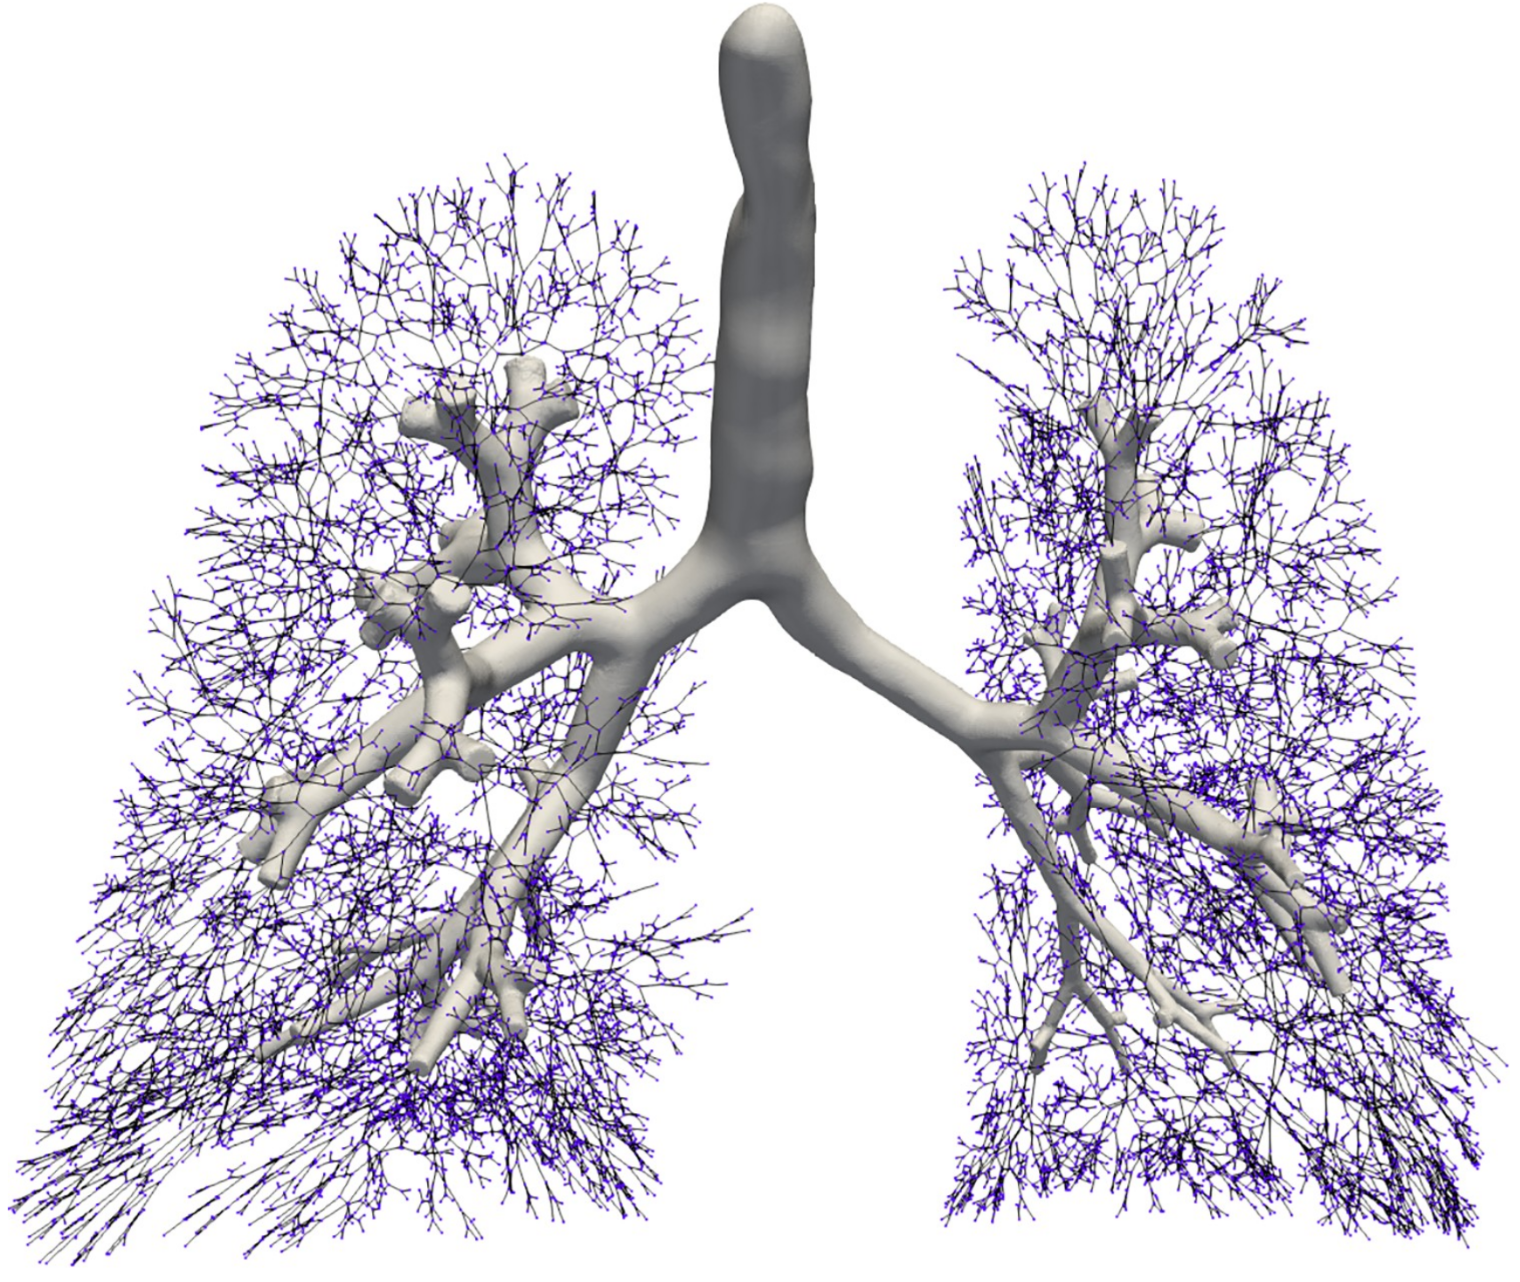
\includegraphics[width=\textwidth]{figures/airway_estimated_12gen.png}  % 12 generations
    \par\small (a) 12 generations        % panel label
  \end{minipage}\hfill                   % space between the panels
  \begin{minipage}[b]{0.49\textwidth}    % right panel
    \centering                           % center inside the panel
    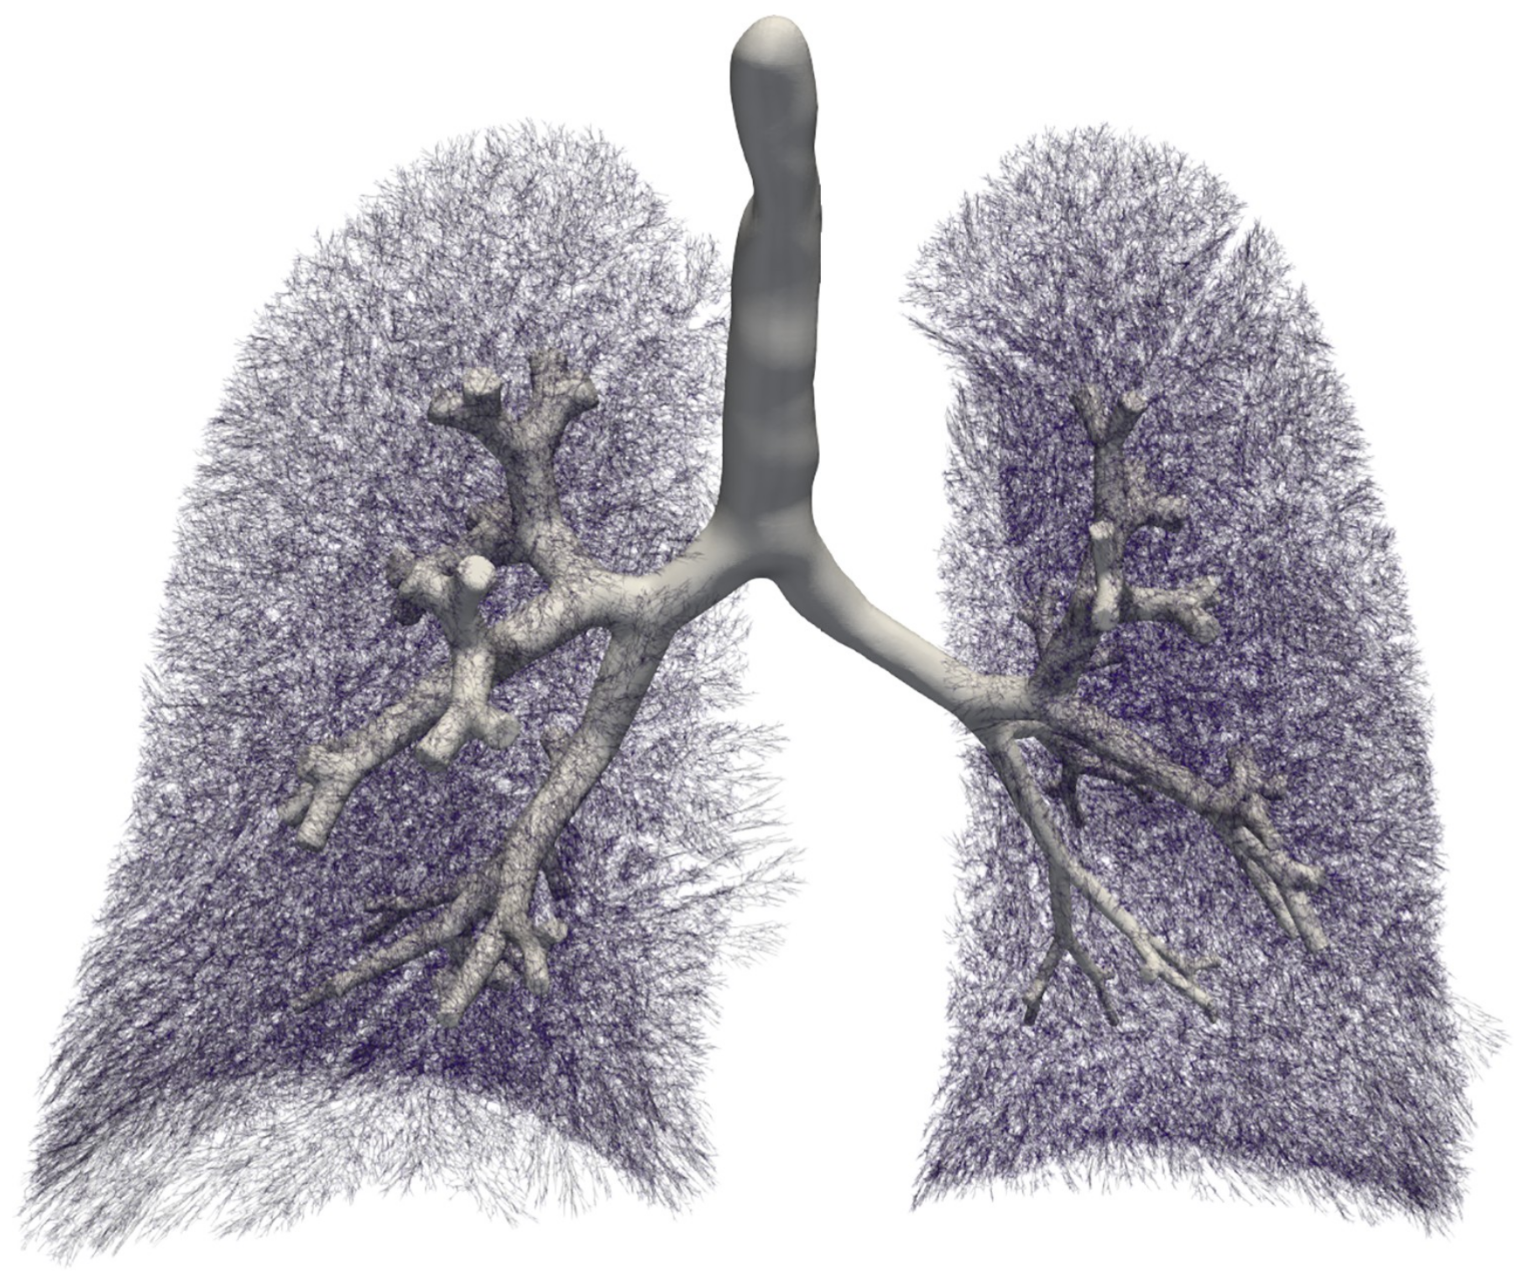
\includegraphics[width=\textwidth]{figures/airway_estimated_23gen.png}  % 23 generations
    \par\small (b) 23 generations        % panel label
  \end{minipage}
  \caption{Bronchial tree estimated from a CT-derived airway tree up to (a) 12 and (b) 23
           generations. The surface is reconstructed for the first 7 generations; deeper
           generations are shown as centerlines. Reproduced from
           \citet{nousias2020avatree}.}
  \label{fig:anatomy_generations}        % referenced as Figure~\ref{fig:anatomy_generations}
\end{figure}
